\section{函数的极值与最值}
\subsection{函数的极值及其求法}
\begin{definition}[驻点]
设函数\(f\colon[a,b]\to\mathbb{R}\),
\(f \in C[a,b] \cap D(a,b)\).
如果\(f'(x_0)=0\),
则称“\((x_0,f(x_0))\)是\(f\)的\DefineConcept{驻点}(stagnation point)”.
\end{definition}

\begin{definition}[极值点]
设函数\(f\colon D\to\mathbb{R}\),\(x_0 \in D\).

如果\[
	(\exists\delta>0)
	(\forall x \in D)
	\left[
		0<\abs{x-x_0}<\delta
		\implies
		f(x)<f(x_0)
	\right],
\]
那么称“\(f(x_0)\)是函数\(f\)的一个\DefineConcept{极大值}(local maximum)”;
称“\(x_0\)是函数\(f\)的一个\DefineConcept{极大值点}”.

如果\[
	(\exists\delta>0)
	(\forall x \in D)
	\left[
		0<\abs{x-x_0}<\delta
		\implies
		f(x)>f(x_0)
	\right],
\]
那么称“\(f(x_0)\)是函数\(f\)的一个\DefineConcept{极小值}(local minimum)”;
称“\(x_0\)是函数\(f\)的一个\DefineConcept{极小值点}”.

函数的极大值、极小值,统称为函数的\DefineConcept{极值}.
函数的极大值点、极小值点,统称为\DefineConcept{极值点}.
\end{definition}

\begin{theorem}[函数存在极值的必要条件]\label{theorem:微分中值定理.函数存在极值的必要条件}
设函数\(f(x)\)在\(x_0\)可导,且在\(x_0\)取得极值,那么\(f'(x_0)=0\).
\end{theorem}
由此可见,可导函数\(f(x)\)的极值点必定是它的驻点,然而函数的驻点不一定是极值点.
此外,函数在它的导数不存在的点处也可能取得极值.

\begin{theorem}[函数存在极值的第一充分条件]\label{theorem:微分中值定理.函数存在极值的第一充分条件}
设函数\(f(x)\)在\(x_0\)连续,且在\(x_0\)的某去心邻域\(\mathring{U}(x_0,\,\delta)\)内可导.
\begin{enumerate}
	\item 若\(x \in (x_0-\delta,x_0)\)时,\(f'(x)>0\);
	而\(x \in (x_0,x_0+\delta)\)时,\(f'(x)<0\);
	则\(f(x)\)在\(x_0\)处取得极大值.

	\item 若\(x \in (x_0-\delta,x_0)\)时,\(f'(x)<0\);
	而\(x \in (x_0,x_0+\delta)\)时,\(f'(x)>0\);
	则\(f(x)\)在\(x_0\)处取得极小值.

	\item 若\(x \in \mathring{U}(x_0,\,\delta)\)时,
	\(f'(x)\)的符号保持不变,
	则\(f(x)\)在\(x_0\)处没有极值.
\end{enumerate}
\begin{proof}
事实上,就情形1来说,
根据函数单调性的判定法,
函数\(f(x)\)在\((x_0 - \delta,x_0)\)内单调增加,
而在\((x_0,x_0 + \delta)\)内单调减少.
又由于函数\(f(x)\)在\(x_0\)处是连续的,
故当\(x\in\mathring{U}(x_0,\delta)\)时,
总有\(f(x) < f(x_0)\),
所以\(f(x_0)\)是\(f(x)\)的一个极大值.
\begin{figure}[ht]
    \def\subwidth{.5\linewidth}
    \begin{subfigure}[b]{\subwidth}
    \centering
        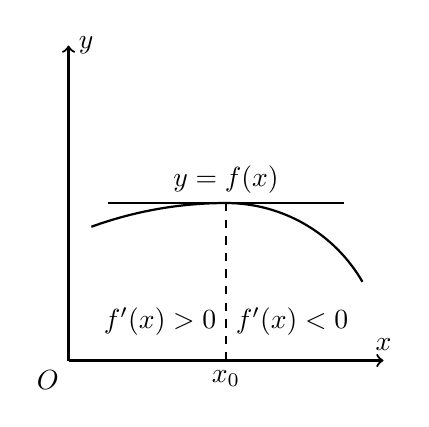
\begin{tikzpicture}
        \draw[thick,->] (0,0) -> (4,0)node[above]{\(x\)};
        \draw[thick,->] (0,0) -> (0,4)node[right]{\(y\)};
        \draw (0,0)node[below left]{\(O\)};
        \draw (2,2)node[above]{\(y=f(x)\)};
        \draw (2,.5)node[left]{\(f'(x)>0\)}node[right]{\(f'(x)<0\)};
        \draw[thick] (2,2)[rotate=90]arc[start angle=0,end angle=-60,radius=2];
        \draw[thick] (2,2)[rotate=90]arc[start angle=0,end angle=20,radius=5];
        \draw (.5,2)--(3.5,2);
        \draw[dashed] (2,2)--(2,0)node[below]{\(x_0\)};
        \end{tikzpicture}
    \subcaption{}
    \end{subfigure}%
    \begin{subfigure}[b]{\subwidth}
    \centering
        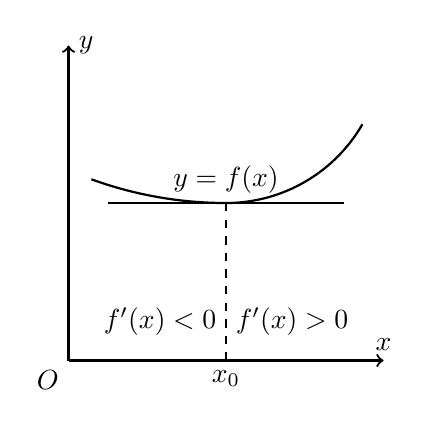
\begin{tikzpicture}
        \draw[thick,->] (0,0) -> (4,0)node[above]{\(x\)};
        \draw[thick,->] (0,0) -> (0,4)node[right]{\(y\)};
        \draw (0,0)node[below left]{\(O\)};
        \draw (2,2)node[above]{\(y=f(x)\)};
        \draw (2,.5)node[left]{\(f'(x)<0\)}node[right]{\(f'(x)>0\)};
        \draw[thick] (2,2)[rotate=-90]arc[start angle=0,end angle=60,radius=2];
        \draw[thick] (2,2)[rotate=-90]arc[start angle=0,end angle=-20,radius=5];
        \draw (.5,2)--(3.5,2);
        \draw[dashed] (2,2)--(2,0)node[below]{\(x_0\)};
        \end{tikzpicture}
    \subcaption{}
    \end{subfigure}%
    \\
    \begin{subfigure}[b]{\subwidth}
    \centering
        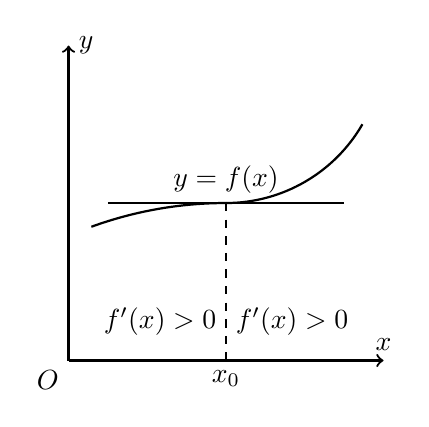
\begin{tikzpicture}
        \draw[thick,->] (0,0) -> (4,0)node[above]{\(x\)};
        \draw[thick,->] (0,0) -> (0,4)node[right]{\(y\)};
        \draw (0,0)node[below left]{\(O\)};
        \draw (2,2)node[above]{\(y=f(x)\)};
        \draw (2,.5)node[left]{\(f'(x)>0\)}node[right]{\(f'(x)>0\)};
        \draw[thick] (2,2)[rotate=-90]arc[start angle=0,end angle=60,radius=2];
        \draw[thick] (2,2)[rotate=90]arc[start angle=0,end angle=20,radius=5];
        \draw (.5,2)--(3.5,2);
        \draw[dashed] (2,2)--(2,0)node[below]{\(x_0\)};
        \end{tikzpicture}
    \subcaption{}
    \end{subfigure}%
    \begin{subfigure}[b]{\subwidth}
    \centering
        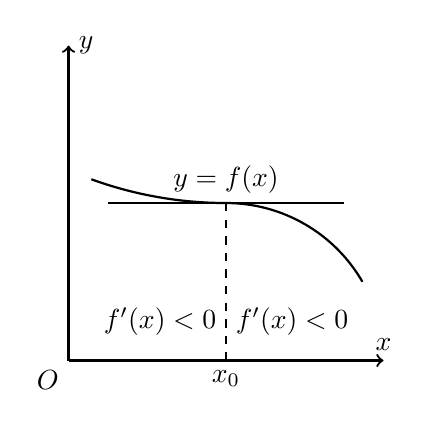
\begin{tikzpicture}
        \draw[thick,->] (0,0) -> (4,0)node[above]{\(x\)};
        \draw[thick,->] (0,0) -> (0,4)node[right]{\(y\)};
        \draw (0,0)node[below left]{\(O\)};
        \draw (2,2)node[above]{\(y=f(x)\)};
        \draw (2,.5)node[left]{\(f'(x)<0\)}node[right]{\(f'(x)<0\)};
        \draw[thick] (2,2)[rotate=90]arc[start angle=0,end angle=-60,radius=2];
        \draw[thick] (2,2)[rotate=-90]arc[start angle=0,end angle=-20,radius=5];
        \draw (.5,2)--(3.5,2);
        \draw[dashed] (2,2)--(2,0)node[below]{\(x_0\)};
        \end{tikzpicture}
    \subcaption{}
    \end{subfigure}%
    \caption{}
\end{figure}

类似地,可证情形2及情形3.
\end{proof}
\end{theorem}
上述定理也可简单地表述为:
当\(x\)在\(x_0\)的邻域内由小及大经过\(x_0\)时,
如果\(f'(x)\)的符号由正变负(即\(f'_-(x_0)>0\)且\(f'_+(x_0)<0\)),
那么\(f(x)\)在\(x_0\)处取得极大值;
如果\(f'(x)\)的符号由负变正(即\(f'_-(x_0)<0\)且\(f'_+(x_0)>0\)),
那么\(f(x)\)在\(x_0\)处取得极小值;
如果\(f'(x)\)的符号并不改变,
那么\(f(x)\)在\(x_0\)处没有极值.

根据\cref{theorem:微分中值定理.函数存在极值的必要条件,theorem:微分中值定理.函数存在极值的第一充分条件},
如果函数\(f(x)\)在所讨论的区间内连续,除个别点歪处处可导,
那么就可以按下列步骤来求\(f(x)\)在该区间内的极值点和相应的极值:
\begin{enumerate}
	\item 求出导数\(f'(x)\);
	\item 求出\(f(x)\)的全部驻点与不可导点;
	\item 考察\(f'(x)\)的符号在每个驻点或不可导点的左右邻域的情形,
	以确定该点是否为极值点;
	如果是极值点,
	进一步确定是极大值点还是极小值点;
	\item 求出各极值点的函数值,就得函数\(f(x)\)的全部极值.
\end{enumerate}

\begin{theorem}[函数存在极值的第二充分条件]\label{theorem:微分中值定理.函数存在极值的第二充分条件}
设函数\(f(x)\)在\(x_0\)处具有二阶导数且\(f'(x_0)=0\),\(f''(x_0)\neq 0\),那么
\begin{enumerate}
	\item 当\(f''(x_0)<0\)时,函数\(f(x)\)在\(x_0\)处取得极大值;
	\item 当\(f''(x_0)>0\)时,函数\(f(x)\)在\(x_0\)处取得极小值.
\end{enumerate}
\end{theorem}
上述定理表明,如果函数\(f(x)\)在驻点\(x_0\)处的二阶导数\(f''(x_0)\neq0\),
那么该驻点\(x_0\)一定是极值点,
并且可以按二阶导数\(f''(x_0)\)的符号来判定\(f(x_0)\)是极大值还是极小值.
但如果\(f''(x_0)=0\),上述定理就不能应用.
事实上,当\(f'(x_0)=0\)且\(f''(x_0)=0\)时,
\(f(x)\)在\(x_0\)处可能有极大值,也可能有极小值,也可能没有极值;
例如,\(f_1(x) = -x^4\),\(f_2(x) = x^4\)和\(f_3(x) = x^3\)
这三个函数在\(x=0\)处就分别属于这三种情况.
因此,如果函数在驻点处的二阶导数为零,
那么还得用一阶导数在驻点左右邻域的符号来判定.

\begin{example}
设函数\(f(x),g(x)\)都具有二阶导数,
且\(g''(x)<0\),\(g(x_0)=a\)是\(g(x)\)的极值,
证明:“\(f'(a)>0\)”是“\(f[g(x)]\)在\(x_0\)取极大值”的充分条件.
\begin{solution}
因为\(g(x_0)=a\)是\(g(x)\)的极值,
所以根据\cref{theorem:微分中值定理.函数存在极值的必要条件}
必有\(g'(x_0)=0\).

记\(F(x) = f[g(x)]\),则\(F'(x) = \eval{f'(u)}_{u=g(x)} \cdot g'(x)\),
\(F''(x) = \eval{f''(u)}_{u=g(x)} \cdot g'(x) \cdot g'(x)
+ \eval{f'(u)}_{u=g(x)} \cdot g''(x)\).
根据\cref{theorem:微分中值定理.函数存在极值的第二充分条件},
要使“\(F(x)=f[g(x)]\)在\(x_0\)取极大值”,只需令\(F''(x_0) < 0\),
那么有\[
	\eval{f'(u_0)}_{u_0=g(x_0)} \cdot g''(x_0) < 0.
\]
由题可知\(g''(x)<0\),
故\(\eval{f'(u_0)}_{u_0=g(x_0)} = f'(a) > 0\),
也就是说“\(f'(a)>0\)”是“\(f[g(x)]\)在\(x_0\)取极大值”的充分条件.
\end{solution}
\end{example}

\subsection{最大值最小值问题}
假定函数\(f(x)\)在闭区间\([a,b]\)上连续,
在开区间\((a,b)\)内除有限个点外可导,
且至多有有限个驻点.
在上述条件下,我们来讨论\(f(x)\)在\([a,b]\)上的最大值和最小值的求法.

首先由闭区间上连续函数的性质,
可知\(f(x)\)在\([a,b]\)上的最大值和最小值一定存在.

其次,如果最大值(或最小值)\(f(x_0)\)在开区间\((a,b)\)内的点\(x_0\)处取得,
那么,按\(f(x)\)在开区间内除有限个点外可导且至多有有限个驻点的假定,
可知\(f(x_0)\)一定也是\(f(x)\)的极大值(或极小值),
从而\(x_0\)一定是\(f(x)\)的驻点或不可导点.
又\(f(x)\)的最大值和最小值也可能在区间的端点处取得.

可用如下的方法求\(f(x)\)在\([a,b]\)上的最大值和最小值:
\begin{enumerate}
	\item 求出\(f(x)\)在\((a,b)\)内的
	驻点\(\AutoTuple{x}{m}\)和不可导点\(x'_1,x'_2,\dotsc,x'_n\);
	\item 计算\(f(x_i)\ (i=1,2,\dotsc,m)\)
	和\(f(x'_j)\ (j=1,2,\dotsc,n)\),
	以及\(f(a)\)和\(f(b)\);
	\item 比较上一步中求出的各个函数值,
	其中最大的就是\(f(x)\)在\([a,b]\)上的最大值,
	最小的就是\(f(x)\)在\([a,b]\)上的最小值.
\end{enumerate}

在求函数的最大值(或最小值)时,特别值得指出的是下述情形:
\(f(x)\)在一个区间(不论有限区间还是无限区间,开区间或闭区间)内可导,
且只有一个驻点\(x_0\),并且这个驻点\(x_0\)是函数\(f(x)\)的极值点,
那么,当\(f(x_0)\)是极大值时,\(f(x_0)\)就是\(f(x)\)在该区间上的最大值;
当\(f(x_0)\)是极小值时,\(f(x_0)\)就是\(f(x)\)在该区间上的最小值.
